\documentclass[11pt]{amsart}
\usepackage{amsmath,amssymb,amsthm,mathtools,enumitem}
\usepackage[margin=1in]{geometry}
\usepackage{hyperref}
\usepackage{graphicx}

\newtheorem{theorem}{Theorem}[section]
\newtheorem{proposition}[theorem]{Proposition}
\newtheorem{corollary}[theorem]{Corollary}
\theoremstyle{remark}
\newtheorem*{remark}{Remark}

\title{The Cutting Plane: Every Line Through the Multiplication Table Is a Conic Section}
\author{Jeremy Ebert}
\address{Franklin County, Ohio, USA}
\date{2026}

\begin{document}
\maketitle

\begin{abstract}
Write out the ordinary multiplication table and draw a straight line through it. What curve does that line trace, once factor pairs are plotted in coordinates built from their sum, difference, and geometric mean? We classify the resulting sections completely: ellipse, parabola, or hyperbola according to the sign of the line coefficients. Anti-diagonals give circles and individual rows or columns give parabolas. We also isolate an exact tangency between every row/column parabola and the anti-diagonal circle whose diameter equals the fixed factor level, and give the true semi-axes and eccentricity of the general ellipse section. The same coordinates restate Fermat factorization and reorganize the classical Dirichlet divisor summatory identity around nested diagonal gnomons.
\end{abstract}

\section{Introduction}
Figure~\ref{fig:table_line} is the geometric picture behind the paper. Panel (b) is the ordinary multiplication table written in the coordinates
\[
X=\frac{x-y}{2},\qquad T=\frac{x+y}{2},
\]
so the usual square grid appears as a triangular side view of a cone. Every cell still represents the ordinary product $xy$. The outer boundary is the anti-diagonal $x+y=12$, while the dashed line $x+y=8$ passes through the factor cells $(2,6)$, $(4,4)$, and $(6,2)$.

Adding
\[
Y=\sqrt{xy}
\]
gives the identity
\[
X^2+Y^2=T^2,
\]
so every factor pair lies on the cone in panel (c). Anti-diagonals $x+y=K$ become fixed-$T$ circles. A general line $ax+by=c$ becomes a cutting plane, and its intersection with the cone is a conic section. The reflected pair
\[
8x+4y=32,\qquad 4x+8y=32
\]
is shown throughout the figure as a concrete example: in the side view these are straight cutting lines; in the flat $(X,Y)$ projection they become mirror ellipses; and in three dimensions they are literally plane sections of the cone.

The emphasis here is deliberately geometric and elementary. Arithmetic structures that can subsequently act on this cone are treated in companion work; none is required for the conic classification, the tangency theorem, the ellipse metric formulas, or the divisor count below.

\begin{figure}[ht]
\centering
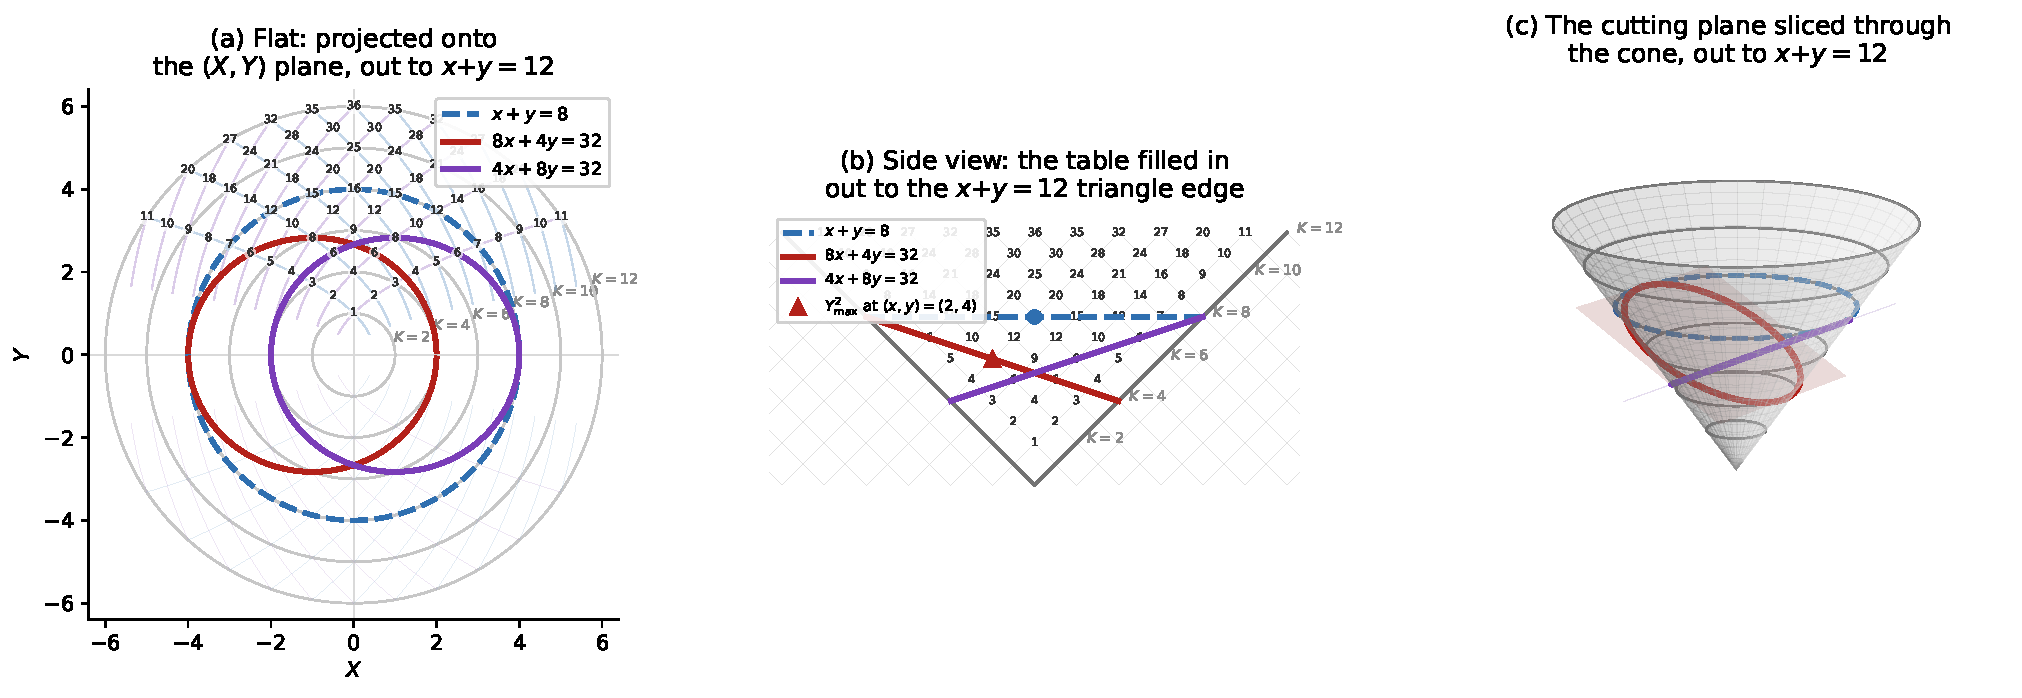
\includegraphics[width=\textwidth]{fig_cutting_plane_3panel.pdf}
\caption{Three views of the same factor geometry, bounded by the anti-diagonal $x+y=12$. (a) Flat $(X,Y)$ projection: fixed sums $x+y=K$ are concentric circles, the row and column families appear as mirror parabolas, the dashed circle is $x+y=8$, and the red/purple cuts are the mirror ellipses arising from $8x+4y=32$ and $4x+8y=32$. (b) Side view in $(X,T)$: the multiplication table becomes a triangular lattice on the cone side view; $x+y=8$ is the horizontal segment $T=4$, while the two example cuts are straight lines. (c) Full cone $X^2+Y^2=T^2$: the same two lines lift to planes whose intersections with the cone are the two ellipses. The figure is illustrative; all classifications and metric statements are proved algebraically below.}
\label{fig:table_line}
\end{figure}

\section{Mean-Value Coordinates and the Conic Identity}
For $x,y>0$ define
\begin{equation}
X=\frac{x-y}2,\qquad Y=\sqrt{xy},\qquad T=\frac{x+y}2. \tag{2.1}
\end{equation}
Then
\begin{equation}
X^2+Y^2=T^2. \tag{2.2}
\end{equation}
Fixing $x+y=K$ fixes $T=K/2$, so the anti-diagonal is represented by the circle
\[
X^2+Y^2=(K/2)^2.
\]
The factor-exchange involution $(x,y)\mapsto(y,x)$ acts simply as
\[
(X,Y,T)\mapsto(-X,Y,T).
\]

\section{The General Conic Theorem}
\begin{theorem}\label{thm:conic}
Let $a,b$ be real numbers, not both zero, and let $ax+by=c$ meet the positive factor quadrant. On $X^2+Y^2=T^2$ it traces an ellipse when $ab>0$, a parabola when $ab=0$, and a hyperbola when $ab<0$. For $a=b$ the ellipse is the anti-diagonal circle.
\end{theorem}
\begin{proof}
For $b\ne0$, $y=(c-ax)/b$, hence
\[
Y^2=xy=\frac cbx-\frac abx^2.
\]
The sign of the quadratic coefficient $-a/b$ gives the three cases. The cases $a=0$ or $b=0$ are the row/column parabolas below.
\end{proof}

\begin{proposition}[Rows and columns]\label{prop:rows}
For a fixed row $x=u$,
\[
X+T=u,\qquad Y^2=u(T-X)=u^2-2uX.
\]
For a fixed column $y=u$,
\[
T-X=u,\qquad Y^2=u(T+X)=u^2+2uX.
\]
Their flat $(X,Y)$ projections are mirror parabolas.
\end{proposition}

\begin{proposition}[Anti-diagonal tangency]\label{prop:tangent}
For every $u>0$, the row and column parabolas at factor level $u$ are tangent in the $(X,Y)$ projection to the same anti-diagonal circle
\[
C_{u/2}:\quad X^2+Y^2=(u/2)^2.
\]
The row is tangent at $(X,Y)=(u/2,0)$ and the column at $(-u/2,0)$. Equivalently, both tangent points lie on the cone slice $T=u/2$ and on its two null generators $X=\pm T$, $Y=0$.
\end{proposition}
\begin{proof}
The row projection is $Y^2=u^2-2uX$, whose vertex is $(u/2,0)$; the column projection is $Y^2=u^2+2uX$, whose vertex is $(-u/2,0)$. Each vertex lies on $C_{u/2}$. Implicit differentiation shows that each parabola and its circle have the same vertical tangent at the corresponding vertex.
\end{proof}

\begin{remark}
Factor level $u$ therefore corresponds exactly to tangent-circle radius $T=u/2$. Consequently a factor mesh of spacing $1/m$ induces a tangent-circle radius mesh of spacing $1/(2m)$. This is a geometric statement about the coordinate map, not an arithmetic invariance claim.
\end{remark}

\begin{proposition}[Coordinate maximum of an ellipse]\label{prop:semiaxes}
For $ab>0$, $Y^2$ is maximized at $x=c/(2a)$, where
\[
Y_{\max}^2=\frac{c^2}{4ab}.
\]
This point is the midpoint of the line's two axis intercepts in factor coordinates.
\end{proposition}
\begin{proof}
Differentiate $Y^2=(c/b)x-(a/b)x^2$ and set the derivative to zero. Substitution gives the stated maximum.
\end{proof}

For the red cut in Figure~\ref{fig:table_line}, $8x+4y=32$, Proposition~\ref{prop:semiaxes} gives the maximum at
\[
(x,y)=(2,4),\qquad Y^2_{\max}=8,
\]
which is the marked point in the side view. The purple cut is its factor-exchange reflection.

\begin{proposition}[True ellipse axes and eccentricity]\label{prop:trueaxes}
For $ab>0$, the ellipse cut from the cone by $ax+by=c$ has semi-minor axis
\[
b_{\rm semi}=\frac{c}{2\sqrt{ab}},
\]
semi-major axis
\[
a_{\rm semi}=\frac{c\sqrt{2(a^2+b^2)}}{4ab},
\]
and eccentricity
\[
e=\frac{|a-b|}{\sqrt{a^2+b^2}}.
\]
In particular the eccentricity depends only on the slope ratio $a/b$, not on the scale $c$, and $e=0$ exactly for the anti-diagonal case $a=b$.
\end{proposition}
\begin{proof}
The section is symmetric under $Y\mapsto-Y$. Its pure-$Y$ semi-axis is $Y_{\max}=c/(2\sqrt{ab})$. At $Y=0$ the two endpoints correspond to factor intercepts $(c/a,0)$ and $(0,c/b)$, hence to cone points
\[
\left(\frac{c}{2a},0,\frac{c}{2a}\right),\qquad
\left(-\frac{c}{2b},0,\frac{c}{2b}\right).
\]
Their Euclidean distance is the full major axis, giving the stated $a_{\rm semi}$. Finally $e^2=1-b_{\rm semi}^2/a_{\rm semi}^2$ simplifies to $(a-b)^2/(a^2+b^2)$.
\end{proof}

For $8x+4y=32$ these formulas give
\[
a_{\rm semi}=\sqrt{10},\qquad b_{\rm semi}=2\sqrt2,\qquad e=\frac1{\sqrt5}.
\]
The mirror cut has the same metric data, as it must.

\begin{remark}
The conic classification itself is a special case of the classical plane-section theorem for a quadric. The contribution here is the explicit factor-coordinate dictionary: the sign of $ab$ classifies the section, the coefficients determine the ellipse geometry above, and the row/column family carries the exact tangent-circle correspondence of Proposition~\ref{prop:tangent}.
\end{remark}

\section{Constant-Product Curves and Fermat Factorization}
Fixing $xy=N$ fixes $Y^2=N$, so
\begin{equation}
T^2-X^2=N. \tag{4.1}
\end{equation}
For odd $N$, Fermat's method searches integers $T\ge\lceil\sqrt N\rceil$ until $T^2-N=X^2$, at which point
\[
N=(T-X)(T+X).
\]
Thus the constant-product hyperbola records the same factorization search directly in the mean-value coordinates.

\section{The Divisor Summatory Function via Nested Gnomons}
Let
\[
D(n)=\sum_{k=1}^n d(k)=\#\{(x,y)\in\mathbb Z_{\ge1}^2:xy\le n\}.
\]
For each diagonal vertex $(u,u)$, $1\le u\le\lfloor\sqrt n\rfloor$, the horizontal and vertical arms terminate at the constant-product boundary. Their integer arm length is $\lfloor n/u\rfloor-u$. Hence
\begin{equation}
D(n)=\sum_{u=1}^{\lfloor\sqrt n\rfloor}\left[2\left(\left\lfloor\frac nu\right\rfloor-u\right)+1\right], \tag{5.1}
\end{equation}
and therefore
\begin{equation}
D(n)=2\sum_{u=1}^{\lfloor\sqrt n\rfloor}\left\lfloor\frac nu\right\rfloor-\lfloor\sqrt n\rfloor^2. \tag{5.2}
\end{equation}
This is the classical symmetric Dirichlet hyperbola identity, now read as nested gnomons whose arms are pieces of the row/column parabolas cut off by $xy=n$.

\section{Discussion}
The cone identity organizes three elementary structures on one carrier: linear conditions become conic sections, constant products become Lorentz-type hyperbolas, and the divisor summatory region decomposes into diagonal gnomons. Proposition~\ref{prop:tangent} adds an exact bridge between the visual layers: each fixed factor level determines both a row/column parabola and a unique tangent anti-diagonal circle of radius $u/2$. Propositions~\ref{prop:semiaxes} and~\ref{prop:trueaxes} retain the full metric information of the general ellipse section.

Figure~\ref{fig:table_line} is therefore not a separate heuristic picture but a compact visualization of the same exact dictionary proved in the text: factor cells, circles, row/column parabolas, cutting lines, and cutting planes are different views of the same coordinate map.

This is the natural stopping point for the geometric paper. Later arithmetic or operator constructions may use the same cone and its two generator rays, but they should be cited as companion results rather than imported into the proof of the elementary statements above.

\begin{thebibliography}{9}
\bibitem{Dickson} L.~E.~Dickson, \emph{History of the Theory of Numbers, Vol.~I}, Carnegie Institution, 1919, Ch.~14.
\bibitem{Dirichlet} P.~G.~L.~Dirichlet, \"Uber die Bestimmung der mittleren Werthe in der Zahlentheorie, \emph{Abh. K\"onigl. Preuss. Akad. Wiss.} (1849), 69--83.
\end{thebibliography}
\end{document}
